\chapter{Discussion}
This chapter servers to discuss the developed solutions and the results from different aspects. Problems, which occured during the bachlor thesis, are presented as well.
\section{Cell as a sphere}
To draw a cell as sphere out of voxels is one way to get the desired spherish shape of the cell. Sadly to keep the shape of the cell during the growth process does not work. Because for a given volume and a given surface there are all kinds of shapes \ac{CC3D} does not know which shape the cell should have. It it suprising that every time the cells get a cubish form during the growth process. It might be a result of the square lattice, which is used in the simulation. There are several research papers, which use \ac{CC3D} for their simulation, sadly it is never explained how the desired cell form is achieved neither which lattice type is used. So far, it is not possible to know if there is an mistake in the simulation or if the cells get a cubish form due to the square lattice. \newline
It is possible that a cell reaches a desired volume and surface, by only setting the terms for the volume and surface of the effective energy. The desired values can be reached faster if a high multiplier, $\lambda_{vol}$ and $\lambda_{sur}$, is set. This has the disadvantage that a volume or an surface constraint might weigh more than the term of the adhesion in the effective energy. If the specific multiplier has a small value, it might be possible that it takes a long time until the desired shape is reached. In addition to the volume and surface constraint comes the adhesion. Because it was one the tasks to find a useful adhesion between cell types for the simulation it has it own paragraph.\newline
\textbf{Other types of cell growth - Angelo tested several}
\section{Adhesion}
Adhesion influences the shape of two or more cells, as it describes how strong the stick to each other. If the adhesion is set too high the cells infiltrate each other but if it is too low the cells may not stick to each other as they change their shape. During the simulations it was observable that some cells of different cell types want to infiltrate each other. This is a result of to high adhesion.
\section{Voxel Density}
In the simulations the voxel density should be set to 1. In this case, in \ac{CC3D} one \SI{1}{\micro\metre} is presented by one voxel. If the voxel density is higher than one voxel represents less \SI{}{\micro\metre}. Because the simulations requires a lot of more time if the voxel density is high and the deviation between the volume and surface values of a cell as a sphere out of voxels and a real sphere is larger, it should be tried to keep the voxel density as small as possible but also not to small. If the voxel density is too small than less details can be displayed and it is much more likely that the cells do not look like spheres. Why the deviation of a cell and a real sphere grows so much more for a higher voxel density is a puzzle. \newline
On one hand the deviation grows with the radius, with more voxels. Since with a higher voxel density there are also more voxels to display it might is a result that \ac{CC3D} uses more voxels to display the cell. On the other hand the volume and surface values of the drawn cell are that high that for the surface of a real sphere a factor of 6 would give an approximation to the surface of the drawn cell. \newline
\section{Deviation of Volume and Surface between a sphere and a cell as sphere}
As it is displayed in figure \ref{img:DeviationSphereCellRealSphere-vD2} the volume of a real sphere and of a drawn sphere cell in \ac{CC3D}, drawn in a simulation with a voxel density of 2, is way to far apart as this voxel density could be used for a realistic simulation of the urothelium. It is interesting to observe that the volume of a sphere cell increases this fast, whereas the surface of a sphere grows in an almost linear way for an increasing radius. Since in \ac{CC3D} in a 3D simulation the volume refers to a physical volume and the surface refers to a physical surface it might be that one voxel still represent \SI{1}{\micro\metre}, even it should be only \SI{0.5}{\micro\metre}. This might explain the results, as they are similiar to the results of $2 \cdot r$ if the voxel densitiy equals 1.
\begin{figure}
	\center
	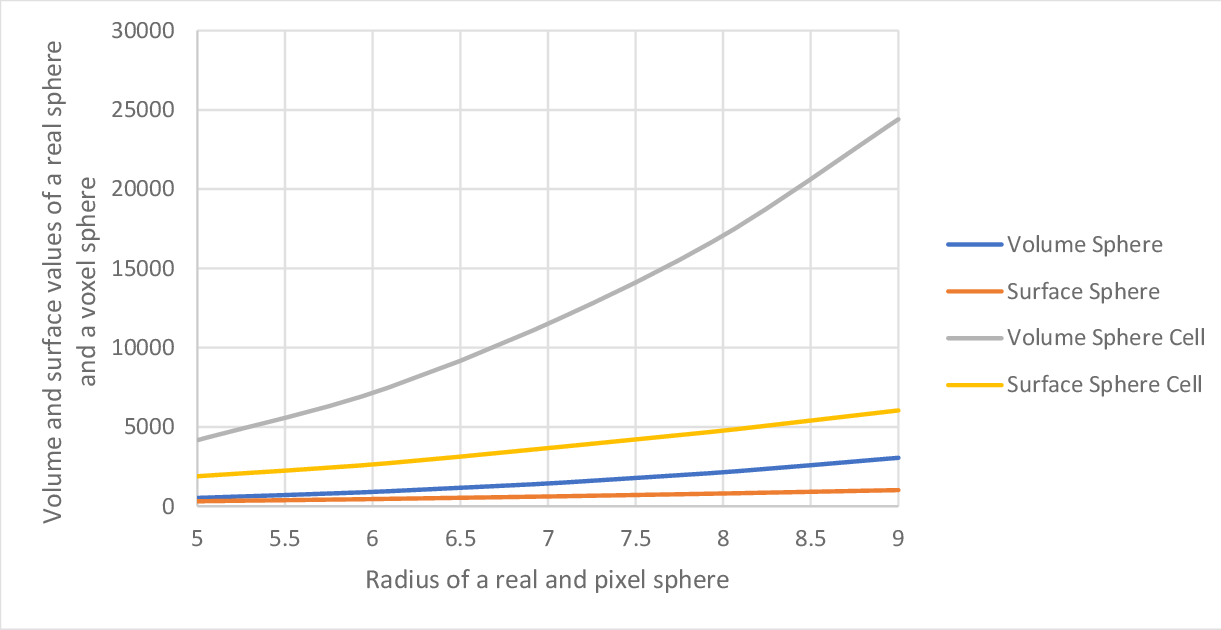
\includegraphics[scale=0.3]{figures/DeviationSphereToPixelSphere-vD2.png}
	\caption{}
	\label{img:DeviationSphereCellRealSphere-vD2}
\end{figure}

\begin{figure}
	\center
	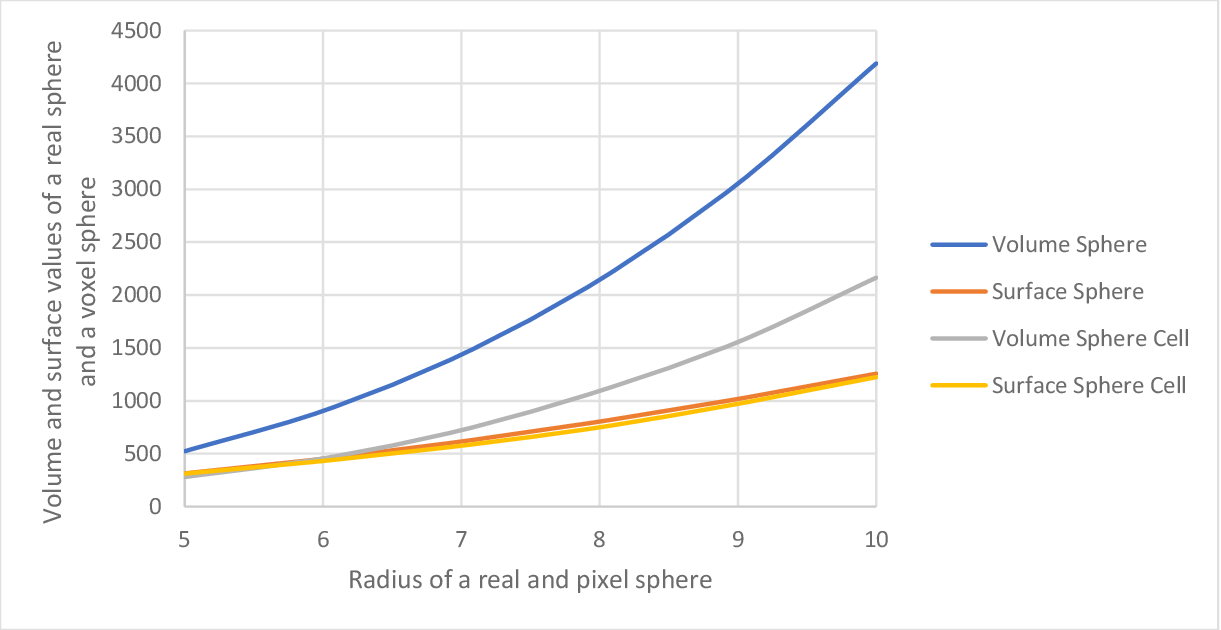
\includegraphics[scale=0.3]{figures/DeviationSphereToPixelSphere-vD0_8.png}
	\caption{}
	\label{img:DeviationSphereCellRealSphere-vD0,8}
\end{figure}

\section{Surface approximation}
The approximation of the surface of a cell to a surface of a real sphere is done with voxels, because these are also used in the simulation field. There are other techniques to approximate the surface of a sphere. It is possible to use pyramids for this approximation. Since in the current simulation the square lattice is used it might is difficult to find an approximation technique which suits the square lattice better. Moreover, the volumes of the cells and of a sphere are almost identical for the same radius, if the voxel density is 1. Because the volume of a cell is more important than the correct surface ,as it is listed in table \ref{tbl:CellConstraints} at page \pageref{tbl:CellConstraints}, a new approximatino has to be checked against its volume as well as its surface. The use of pyramids might be in general a great way to approximate a sphere but for the square lattice it might be not as suited as the use of cuboids.

\section{Surface Variation Pixels to Sphere}
The created algorithm of section \ref{sec:CreatedAlgorithm} has its benefits and also its weaknesses. There are several ways to design the algorithm. One is to use the same method as it is used to draw the sphere cell. With this method every voxel in the cuboid has to be checked if it is inside or outside the algorithm. Therefore, a lot of calculations are required just to create the matrix from which the volume and surface sites can be calculated. This amount of calculations is $r^{3}$, where the radius of the cuboid is $2 \cdot r$, as it is explained in section \ref{sec:DrawSphereCells}. Thus, the amount of calculations to create the algorithm is $(2 \cdot r)^{3}$, where $r$ is the radius of the sphere. Because this approach has a high computational cost it should be only used if it is necessary. \newline
The next two approaches are similiar. Both split the cuboid and the circle up into 8 pieces, then the calculations are done with one of the 8 cuboids and as last step this result gets mirrored. This is possible because a cuboid split up into an odd amount of parts creates several smaller cuboids. With this small cuboid it is possible to calculate if every cuboid, in the small cuboid, is inside the sphere. Then the matrix is created. For the calculation of the volume and surface the result of the one eigth of the cuboid is mirrored for all three axes. This approach has less computations than the approach before. The amount of computations is now $(\dfrac{r}{2})^{3}$. Because only the half of the radius of the sphere is used, this is an improvement over the approach before. \newline
The approach with the least computational cost is similiar to the one before. After the cuboid around the sphere is split up into 8 pices, the point in which the circle is at a given x,z coordinate is calculated. Then it is checked which cuboids at this given x,z coordinate are within the circle or not. Based on this approach there are even less calculations. Because of the eigth of the cuboid only the height of the circle for a given x,z coordinate is calculated. The required amount of calculations is now $(\dfrac{r}{2})^{2})$. Because one eigth of the cuboid is used, the half of the radius of the sphere is required. Moreover, only every x,z coordinate is needed for the calculations, instead of every x,y,z coordinate of the cuboids. Thus, the approach of the algorithm has the lowest computational cost. Even the algorithm has its weakness, it might be further developed.

\section{CC3D}
Several simulation programs have been tested in an earlier master thesis of the project \ref{MA Angelo}, it was evidenced that \ac{CC3D} is the best suited program. During this bachelor thesis I realized several weaknesses of \ac{CC3D} which are explained in the following paragraph. \newline
To develop a program an debugger should be available. An debugger allows the developer to execute the program command wise and to observe the values of the variables. \ac{CC3D} do not offer an debugger. Therefore every observation of a variable or the order of the function calls has to be printed to the command line. This has signifacant disadvantages, as it requires more time to understand the structure of the code as well as the print commands first have to be written. Moreover, the developer has to be very precise at the print commands and she / he needs to know which output at the command line belongs to which print command. \newline
A second disadvantage is that the memory after an simulation is not released. Every simulation requires an specific amount of memory dependent of the simulation field size. This memory should be released after the simulation is finished. If the memory would be released after the simulation other programs could use it. Moreover, by starting a simulation after another simulation is finished, \ac{CC3D} reserves the memory for the new simulation in addition to the required simulation before. Therefore, by starting several simulations without closing \ac{CC3D}, the program has a high probability to crash because there is not enough memory free for the simulation. \newline
Because the required memory for an simulation increases as the size of the simulation field increases it is good to know where the constraints of the size of the simulation field are. The size constraints was tested on an \ac{VM} with the distribution 'windows 7' as an 64 bit version. The \ac{VM} has a memory of 4GB. For this memory the constraint of the size of the simulation field is around by 400 voxels for each axis. Therefore, around 107171875 voxels are allowed in the simulation. For this size of the simulation field \ac{CC3D} became very slow, which is a result of the amount of memory. This constraint is different for different distributions as well as for different sizes of the memory. 

\section{GGH Model}
The \ac{GGH} model is widely used because it is easy to use. Even it is easy to use some parameters of the approach are not explained in detailed. As example it is possible to set a temperature for the simulation. This temperature effects how much a cell fluctuates as it changes its volume or surface. That the fluctuations changes with a different temperature is observable. Because it is almost nowhere explained it is questionable if this is the only effect of the temperature in the simulation or are the other effects with it. \newline
For the scenario with the sphere cell it is a disadvantage that it is not possible to set a constraint of the shape of a cell. The use of one radius or one diameter would already be enough to limit the amount of possible shapes of a cell for a given volume and surface. Because such a constraint can not be set and it is not explained in the literautre how to receive a specific shape of a cell a lot of experiments has to be done to reach the desired shape of the cell.